\documentclass{scrbook}
\usepackage[ngerman]{babel}
\usepackage[T1]{fontenc}
\usepackage[ansinew]{inputenc}
\usepackage{a4wide}

%verwenden von grafiken
\usepackage[dvipdf, final]{graphicx}

%verwenden von hyperlinks, stil derselben
\usepackage{color}
\definecolor{darkblue}{rgb}{0,0,0.5}

\usepackage{hyperref}
\hypersetup{
%	draft,										%hyperlinks ausschalten				
	colorlinks,									%hyperlinks farbig darstellen
	linkcolor   = darkblue,
	filecolor   = darkblue,
	urlcolor    = darkblue,
	citecolor   = darkblue,
	pdftitle    = {Handbuch},	%titel
	pdfsubject  = {j-Algo},			%thema
	pdfauthor   = {Alexander Claus, Matthias Schmidt},
	pdfkeywords = {Algorithmen, Visualisierung},
	pdfcreator  = {Distiller},
	pdfproducer = {LaTeX mit Hyperref-Package}}

%spezielle kommandos
%schreibweise des software-titels
\newcommand{\jalgo}{\mbox{\bfseries {\color{red}j}-Algo} }
%pfad zu den bildern
\newcommand{\pfad}{pics/}
%f�gt ein bild an einer bestimmten stelle, relativ zur position des befehls, ein.
%usage: \icon{dateiname}{y-offset}{x-offset}{bildvergr��erung}
\newcommand{\icon}[4]{
	\vspace{#2 ex}
	\hspace{#3 ex}
	\includegraphics[scale=#4]{\pfad #1}
}
%f�gt ein bild mittig mit bildunterschrift ein.
%usage: \centerpic{dateiname}{bildvergr��erung}{untertitel}
\newcommand{\centerpic}[3]{
	\begin{center}
		\includegraphics[scale=#2]{\pfad #1}\\
		{\small #3}
	\end{center}
}
%f�gt eine \subsection mit einem f�hrenden icon ein
%usage: \subsectionicon{text}{icon}
\newcommand{\subsectionicon}[2]{
	\subsection[#1]{\qquad #1}
	\icon{#2}{-5}{7}{1}
	\\
}
%f�gt eine \subsection mit 2 f�hrenden icons ein
%usage: \subsectiondoubleicon{text}{icon1}{icon2}
\newcommand{\subsectiondoubleicon}[3]{
	\subsection[#1]{\qquad \quad #1}
	\icon{#2}{-5}{7}{1}
	\icon{#3}{0}{-2}{1}
	\\
}
%f�gt eine \subsubsection* mit 2 f�hrenden icons ein
%usage: \subsubsectiondoubleicon{text}{icon1}{icon2}
\newcommand{\subsubsectiondoubleicon}[3]{
	\subsubsection*{\qquad \qquad #1}
	\icon{#2}{-4}{1}{1}
	\icon{#3}{0}{-2}{1}
	\\
}

\begin{document}

\begin{titlepage}
\centerpic{main/title}{1}{}
\vfill
\begin{flushright}
{\Huge \textbf{Benutzerhandbuch}}
\end{flushright}
\end{titlepage}

\newpage

\tableofcontents
\newpage

\part{Das Hauptprogramm}
\section{Einleitung}
Dieses Handbuch soll k�nftigen Entwicklern von \jalgo helfen, sich schnell mit der Struktur der Software auseinanderzusetzen. \jalgo ist eine Software, die sich mit der Visualisierung von Algorithmen besch�ftigt. Sie soll dazu dienen, verschiedene Algorithmen zu veranschaulichen um sie so Studenten und anderen Interessierten verst�ndlicher zu machen. Die Anwendung basiert auf einer Plugin-Struktur, die es erm�glicht, einzelne Module, die jeweils einen Algorithmus oder ein Themengebiet abdecken k�nnen, in das Programm zu integrieren und zu laden.

Sowohl \jalgo als auch die einzelnen Module entstanden im Rahmen des externen Softwarepraktikums im Studiengang Informatik der TU Dresden in Zusammenarbeit mit dem Lehrstuhl Programmierung. Die implementierten Module orientieren sich daher an den Lehrveranstaltungen "`Algorithmen und Datenstrukturen"' sowie "`Programmierung"' im Grundstudium Informatik an der TU Dresden. Das Einsatzgebiet soll vor allem die Vorlesung und das studentische Lernen zu Hause umfassen.\\
\jalgo ist eine freie Software, die beliebig oft kopiert werden darf.

\bigskip
\section{Technische Hinweise}
\subsection{Systemvoraussetzungen}
Folgende minimale Systemanforderungen werden f�r den reibungslosen Einsatz von \jalgo ben�tigt:
\begin{itemize}
	\item IBM-kompatibler PC 
	\item Mindestens 64 MB RAM
	\item {\sc Windows} 98(SE)/ME/2000/XP , {\sc Linux} SuSE/Red Had 	
	\item Java 2 Platform Standard Edition 5.0 {\small (siehe: \href{http://java.sun.com/}{http://java.sun.com/})}
	\item Maus und Tastatur	
	\item Monitor mit einer Aufl�sung von mindestens 800x600 
\end{itemize}

\medskip
\subsection{Installation}
\subsubsection*{Windows}
Entpacken Sie nach dem Herunterladen das ZIP-komprimierte Archiv in einen Ordner Ihrer Wahl. 
In diesem Ordner finden Sie eine Datei namens "`j-algo.bat"'. 
�ffnen Sie diese Datei mit einem Doppelklick, und das Programm wird gestartet.

\subsubsection*{Unix}
Entpacken Sie nach dem Herunterladen das TGZ-komprimierte Archiv in einen Ordner Ihrer Wahl. 
In diesem Ordner finden Sie eine Datei namens "`j-algo.sh"'. 
�ffnen Sie die Konsole und starten sie mittles \verb|sh j-algo.sh| das Programm.

\medskip
\subsection{Deinstallation}
Der komplette Programmordner kann jederzeit gefahrlos von der Festplatte gel�scht werden.

\newpage
\section{Grundfunktionen}
\jalgo bietet eine Reihe von Grundfunktionen, die unabh�ngig von den Modulen zur Verf�gung stehen, bzw. f�r jedes Modul die gleiche Bedeutung haben. Im Einzelnen sind das das �ffnen von Modulen sowie das Laden und Speichern von Sitzungsdaten. Die Grundfunktionen sind �ber die Werkzeugleiste oder den Men�punkt <\textsc{Datei}> erreichbar.

\subsectionicon{Neues Modul �ffnen}{main/icon_new}
Ein Klick auf den Button <\textsc{Neu}> in der Werkzeugleiste gibt Ihnen die M�glichkeit, ein beliebiges neues Modul zu �ffnen. Dabei wird ein Auswahldialog ge�ffnet, in welchem die installierten Module aufgelistet sind. Hier werden Ihnen au�erdem kurze Informationen zu diesen Modulen angezeigt. Sie k�nnen w�hlen, ob dieser Auswahldialog bei jedem Start des Programmes angezeigt werden soll oder nicht.\\
Alternativ dazu kann �ber das Men� \textsc{<Datei>$\rightarrow$<Neu>} das gew�nschte Modul geladen werden. Dies ist der schnellere Weg und zu empfehlen, wenn man bereits einen �berblick �ber die installierten Module hat.

\subsectionicon{Gespeicherte Sitzungsdaten laden}{main/icon_open}
Mit einem Klick auf den Button <\textsc{�ffnen}> erscheint ein Dialog zur Dateiauswahl. Hier haben Sie die M�glichkeit, eine Datei auszuw�hlen, in welcher modulspezifische Sitzungsdaten gespeichert wurden. Die Dateien, die von \jalgo gespeichert werden, tragen die Dateiendung \emph{"`.jalgo"'}.\\
Achtung: Da jedes Modul von \jalgo seine Daten in einer solchen Datei ablegt, kann man beim Blick auf die unge�ffnete Datei nicht erkennen, mit welchem Modul diese assoziiert wurde. Es wird jeweils das assoziierte Modul zu der geladenen Datei ge�ffnet. Achten Sie daher bei der Vergabe der Dateinamen auf m�glichst eindeutige Bezeichner.\\
Anmerkung: In einer sp�teren Version wird direkt bei der Dateiauswahl das zugeh�rige Modul mit angezeigt.
\centerpic{main/loaddialog}{0.45}{Das Dialogfenster zum �ffnen}

\medskip
\subsectiondoubleicon{Sitzungsdaten speichern}{main/icon_save}{main/icon_save_as}
Per Klick auf die Buttons <\textsc{Speichern}> und <\textsc{Speichern unter}> k�nnen Sie die Sitzungsdaten des gerade aktiven Moduls in einer Datei speichern. Wie beim Laden �ffnet sich auch hier ein Dialog zur Dateiauswahl, in welchem Sie Zielpfad und Name der neuen Datei eintragen k�nnen. Die Angabe der Dateiendung ist nicht n�tig, das Programm 
erg�nzt diese automatisch.\\
Je nach Implementierung des aktiven Moduls steht die Speicherfunktion nur zur Verf�gung, wenn gerade kein Algorithmus l�uft. Sollte noch ein Algorithmus aktiv sein, so beenden Sie diesen bitte vorher oder brechen ihn ab.

\subsection{Modul schlie�en}
Sie haben die M�glichkeit, jede Modulinstanz durch Klick auf das Kreuz der dazugeh�rigen Registerkarte zu schlie�en. Dabei werden Sie gegebenenfalls gefragt, ob Sie Ihre Arbeit speichern wollen. Um das gesamte Programm zu schlie�en, ist es nicht n�tig, die Module einzeln zu schliessen, das erledigt das Programm f�r Sie.

\bigskip
\begin{center}
	\raisebox{-7ex}{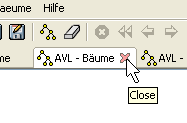
\includegraphics[scale=0.8]{\pfad main/closebutton}} \hfill
	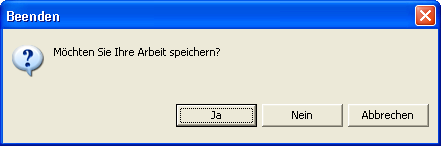
\includegraphics[scale=0.55]{\pfad main/closemessage} \\
	{\small Der Knopf zum Schlie�en eines Moduls.} \hfill
	{\small Die Abfrage, ob die Daten gespeichert werden sollen.}
\end{center}

\subsectionicon{Einstellungen}{main/icon_prefs}
\jalgo bietet ein paar M�glichkeiten an, das Programm den Bed�rfnissen des Benutzers anzupassen. Den Dialog f�r die Grundeinstellungen erreichen Sie unter dem Men�punkt\\ \textsc{<Datei>$\rightarrow$<Einstellungen>}
\centerpic{main/prefsdialog}{0.8}{Der Dialog f�r die Grundeinstellungen}
Unter anderem kann hier die Sprache eingestellt werden. Au�erdem bietet sich die M�glichkeit, die Art der graphischen Oberfl�che zu �ndern, da unter manchen Betriebssystemen diverse Oberfl�chenelemente nicht immer vorteilhaft aussehen.

\subsectionicon{Hilfe}{main/icon_help}
Die Hilfe stellt ein wichtiges Nachschlagewerk f�r all diejenigen dar, die nicht auf Anhieb mit allen Funktionen von \jalgo und seinen Modulen klar kommen. Hier k�nnen Sie noch einmal eine genaue Beschreibung zu den einzelnen Programmelementen nachlesen.\\
Die Hilfe ist kontextspezifisch aufgebaut, d.h. ist ein Modul ge�ffnet, so wird in der Hilfe automatisch an die entsprechende Stelle gesprungen.\\
Sie erreichen die Hilfe �ber den Men�punkt \textsc{<Hilfe>$\rightarrow$<Inhalt>} oder indem Sie einfach auf die Taste <\textsc{F1}> Ihrer Tastatur dr�cken.

\subsection{Hinweis-Tipps}
Zus�tzlich wird zu den meisten Kontrollelementen, also Buttons, Men�eintr�ge, etc., ein kurzer Hinweistext neben dem Mauszeiger bzw. in der Statuszeile des Programmes angezeigt. Dies sollte als schnelle Hilfestellung den meisten Anforderungen gen�gen.

\newpage
\section{Impressum}
Das Modul \ebnf wurde im Sommersemester 2006 von der Praktikumsgruppe 12 im Rahmen des externen Softwarepraktikums entwickelt. Mitwirkende waren die
\paragraph{Teammitglieder}
\begin{itemize}
\item Tom Kazimiers --- Administrator
\item Johannes Mey --- Testverantwortlicher
\item Michael Thiele --- Chefprogrammierer
\item Andr� Viergutz --- Assistent
\item Claas Wilke --- Sekret�r	
	
\end{itemize}
sowie der betreuende Tutor Matthias Schmidt.\\
Die Webseite des Projektes finden Sie unter \href{http://web.inf.tu-dresden.de/~swt06-12/}{http://web.inf.tu-dresden.de/\~{}swt06-12/}.

\newpage
\newpage

\part{Die Module}
\newcommand{\kmp}{\mbox{\bfseries KMP} }


\section{Einleitung}
Dieses Handbuch soll k�nftigen Entwicklern von \jalgo helfen, sich schnell mit der Struktur der Software auseinanderzusetzen. \jalgo ist eine Software, die sich mit der Visualisierung von Algorithmen besch�ftigt. Sie soll dazu dienen, verschiedene Algorithmen zu veranschaulichen um sie so Studenten und anderen Interessierten verst�ndlicher zu machen. Die Anwendung basiert auf einer Plugin-Struktur, die es erm�glicht, einzelne Module, die jeweils einen Algorithmus oder ein Themengebiet abdecken k�nnen, in das Programm zu integrieren und zu laden.

Sowohl \jalgo als auch die einzelnen Module entstanden im Rahmen des externen Softwarepraktikums im Studiengang Informatik der TU Dresden in Zusammenarbeit mit dem Lehrstuhl Programmierung. Die implementierten Module orientieren sich daher an den Lehrveranstaltungen "`Algorithmen und Datenstrukturen"' sowie "`Programmierung"' im Grundstudium Informatik an der TU Dresden. Das Einsatzgebiet soll vor allem die Vorlesung und das studentische Lernen zu Hause umfassen.\\
\jalgo ist eine freie Software, die beliebig oft kopiert werden darf.

\bigskip
\section{Technische Hinweise}
\subsection{Systemvoraussetzungen}
Folgende minimale Systemanforderungen werden f�r den reibungslosen Einsatz von \jalgo ben�tigt:
\begin{itemize}
	\item IBM-kompatibler PC 
	\item Mindestens 64 MB RAM
	\item {\sc Windows} 98(SE)/ME/2000/XP , {\sc Linux} SuSE/Red Had 	
	\item Java 2 Platform Standard Edition 5.0 {\small (siehe: \href{http://java.sun.com/}{http://java.sun.com/})}
	\item Maus und Tastatur	
	\item Monitor mit einer Aufl�sung von mindestens 800x600 
\end{itemize}

\medskip
\subsection{Installation}
\subsubsection*{Windows}
Entpacken Sie nach dem Herunterladen das ZIP-komprimierte Archiv in einen Ordner Ihrer Wahl. 
In diesem Ordner finden Sie eine Datei namens "`j-algo.bat"'. 
�ffnen Sie diese Datei mit einem Doppelklick, und das Programm wird gestartet.

\subsubsection*{Unix}
Entpacken Sie nach dem Herunterladen das TGZ-komprimierte Archiv in einen Ordner Ihrer Wahl. 
In diesem Ordner finden Sie eine Datei namens "`j-algo.sh"'. 
�ffnen Sie die Konsole und starten sie mittles \verb|sh j-algo.sh| das Programm.

\medskip
\subsection{Deinstallation}
Der komplette Programmordner kann jederzeit gefahrlos von der Festplatte gel�scht werden.

\newpage
\section{Der Willkommensbildschirm}
\label{sec:DerWillkommensbildschirm}

\subsection{Modul KMP starten}
\label{sec:ModulKMPStarten}

Nach Starten des Hauptprogramms j-Algo k�nnen Sie �ber den Button 'Neu' oder mit dem Men�punkt 'Datei' => 'Neu' eine neue Instanz des Moduls KMP �ffnen. Anschlie�end �ffnet sich der Willkommensbildschirm des Moduls, der Ihnen verschiedene M�glichkeiten er�ffnet.			
		
\bigskip
\centerpic{kmp/welcomescreen}{0.5}{Der Willkommensbildschirm des Moduls}
\bigskip

\subsectionicon{Generierung der Verschiebetabelle}{kmp/welcome_phaseone}
Mit Klick auf das erste Symbol gelangen Sie zur ersten Phase des KMP-Algorithmus, in dem f�r ein Pattern die Verschiebetabelle erstellt wird.

\subsectionicon{ Suchen im Suchtext}{kmp/welcome_phasetwo} 
Mit Klick auf das zweite Symbol gelangen Sie zur zweiten Phase des KMP-Algorithmus, in dem ein Text nach einem Pattern durchsucht wird.

\subsectionicon{ �ffnen einer KMP-Sitzung}{kmp/welcome_open}  
Mit Klick auf das Ordner-Symbol erhalten Sie die M�glichkeit, ein zuvor gespeichertes KMP-Beispiel zu laden ("*.jalgo" - Datei)

\subsectionicon{ Pr�sentation von Lernbeispielen}{kmp/welcome_example}   
Mit Klick auf das Tafel-Symbol erhalten Sie die M�glichkeit, anhand gegebener repr�sentativer Lernbeispiele die Funktions- und Arbeitsweise des Algorithmus kennenzulernen.
\section{Die Arbeitsfl�che}
Die Arbeit mit \avl spielt sich auf der Arbeitsfl�che ab. Sie bietet alle Funktionalit�ten 
des Moduls und ist in f�nf wichtige Bereiche unterteilt:
\begin{itemize}
	\item \textsc{Zeichenfl�che}\\
		Der Baum und alle Algorithmen werden hier visualisiert.
	\item \textsc{Infobereich}\\
		Wichtige Baumdaten wie Anzahl der Knoten, Baumh�he und Suchtiefe sind hier zu finden.
	\item \textsc{Kontroll-Bereich}\\
		In diesem Bereich erfolgt der Start und die Steuerung der Algorithmen.
	\item \textsc{Dokumentationsbereich}\\
		Hier l�uft der Text zum jeweiligen Algorithmus mit. Der aktuelle Schritt wird dabei farbig hervorgehoben. Der Text ist dem Skript "`Algorithmen, Datenstrukturen und Programmierung"' von Prof. Vogler, Version vom 2. Oktober 2003, entnommen.
	\item \textsc{Logbuch}\\
		Hier werden erfolgte Einzelaktionen protokolliert und dabei der jeweils aktuelle Schritt farbig hervorgehoben.
\end{itemize}

Die Aufteilung zwischen dem unteren und dem oberen Bereich kann mit dem Schiebebalken ver�ndert werden. Per Klick auf die schwarzen Pfeile k�nnen Sie den Textbereich wahlweise maximieren, um einen �berblick �ber den Algorithmustext zu gewinnen, oder minimieren, um die Zeichenfl�che zu vergr��ern.
\newpage
\centerpic{avl/prgmscreen}{1}{Die Arbeitsfl�che des Moduls \avl}
\section{Modulfunktionen}
Alle Funktionen des Moduls \avl lassen sich �ber den Kontroll-Bereich der Arbeitsfl�che bedienen. Sie stellen die verschiedenen Baumalgorithmen dar, deren Visualisierung Aufgabe dieses Moduls ist. Grundlegend l�uft die Arbeit mit den Algorithmen immer nach dem gleichen Schema ab:
\begin{enumerate}
	\item Schl�sseleingabe
	\item Starten des Algorithmus per Klick auf den entsprechenden Button
\end{enumerate}
Es gibt nat�rlich auch Algorithmen, wie der AVL-Test, die keinen Schl�ssel ben�tigen und ohne Schritt 1 auskommen.\\
Es folgen nun die einzelnen Funktionen im Detail. 

\subsection{Schl�sseleingabe}
F�r die Eingabe der Schl�sselwerte steht ein Textfeld und ein Button f�r zuf�llige Werte zur Verf�gung. Es sind nur ganzzahlige Schl�sselwerte von 1 bis 99 erlaubt.\\
�ber dem Textfeld befindet sich eine Nachrichtenzeile, in welcher Sie auf eventuelle Fehleingaben aufmerksam gemacht werden. Hier werden sp�ter ebenfalls kurze Ergebnismeldungen zu den Algorithmen eingeblendet.

\subsection{Algorithmusfunktionen}
\subsubsection*{Knoten einf�gen}
Der eingegebene Wert wird als Schl�ssel f�r einen neuen Knoten verwendet, der in den Baum eingef�gt werden soll. Ist bereits ein Knoten mit dem gleichen Schl�ssel im Baum enthalten, so bricht der Algorithmus erfolglos ab.
\subsubsection*{Knoten suchen}
Nach dem Starten dieses Algorithmus beginnt die Suche nach dem eingegebenen Schl�ssel im Baum.
\subsubsection*{Knoten l�schen}
Nach dem eingegebenen Schl�ssel wird gesucht, und wenn ein entsprechender Knoten gefunden wurde, wird dieser aus der Baumstruktur entfernt.

\subsection{AVL-Modus}
Ist dieses K�stchen aktiviert, werden die entsprechenden Algorithmen so ausgef�hrt, dass die AVL-Eigenschaft gewahrt bleibt.\\
Achtung: Es ist keine Funktion implementiert, die an einem beliebigen Suchbaum die AVL-Eigenschaft herstellt!\\
Ist das K�stchen deaktiviert, ist es daher nicht immer ohne weiteres wieder zu aktivieren. Dazu muss zuerst getestet werden, ob der Baum die AVL-Eigenschaft hat. Es ist jedoch jederzeit m�glich, das K�stchen zu deaktivieren und einen unbalancierten Baum zu erzeugen.

\subsection{Baum auf AVL-Eigenschaft testen}
\medskip
\centerpic{avl/avltest}{1}{Hinweisfenster des AVL-Tests}
Wenn der AVL-Modus einmal deaktiviert sein sollte, so erm�glicht das Programm einen Test des Baumes auf die AVL-Eigenschaft. Dabei erfolgt eine Berechnung und Anzeige der Balancen aller Knoten und das eventuelle Markieren von Knoten, deren Balance sich nicht mehr im Rahmen der AVL-Eigenschaft bewegt.\\
Es wird ein Hinweis-Dialog ge�ffnet, der Ihnen das Ergebnis des Tests pr�sentiert. Sollte der Baum tats�chlich die AVL-Eigenschaft besitzen, so wird Ihnen angeboten, direkt in den AVL-Modus zu wechseln.

\newpage
\subsection{Baum l�schen}
Mit einem Klick auf den Button \raisebox{-1.5ex}{
\includegraphics[scale=1]{\pfad avl/icon_clear}} in der Werkzeugleiste k�nnen Sie nach einer Sicherheitsabfrage die gesamte Baumstruktur l�schen und mit einer leeren Arbeitsfl�che neu beginnen.
\medskip
\centerpic{avl/cleartreemessage}{1}{Sicherheitsabfrage beim L�schen des Baumes}

\vfill
\section{Algorithmussteuerung}
Aufgabe des Moduls \avl ist es, Baumalgorithmen, wie das Einf�gen und L�schen von Knoten, zu visualisieren. Jeder Algorithmus ist in verschiedene Teilschritte unterteilt, die nacheinander angezeigt werden. Das Visualisieren erfolgt dabei durch das Zeichnen des Baumes, durch die Erkl�rung der Schritte im Dokumentationsbereich und im Logbuch und durch die Neuberechnung der baumspezifischen Daten, die im Infobereich pr�sentiert werden.\\
Nachdem Sie einen Algorithmus gestartet haben, verweilt er in einem Initialzustand und wartet auf Ihre Eingabe. Nun haben Sie die M�glichkeit, den Algorithmus in kleinen oder gro�en Schritten zu durchlaufen; Sie k�nnen ihn sofort beenden oder direkt abbrechen. Daf�r bietet die Algorithmussteuerung die entsprechenden Werkzeuge.

\subsection{Schritt-Pfeile}
Mittels der Schritt-Pfeile steuern Sie die Abfolge der Einzelschritte und bekommen so eine detaillierte Sicht auf die Arbeitsweise des Algorithmus. Das Programm bietet Ihnen die M�glichkeit, einen Teilschritt r�ckg�ngig zu machen und damit gewisse Abl�ufe zu wiederholen. Die Schritt-Pfeile, welche die R�ckg�ngigfunktion anbieten, weisen in ihrer Richtung nach links und sind dadurch intuitiv von den Vorw�rts-Pfeilen zu unterscheiden.\\
Zus�tzlich gibt es f�r jede Richtung einen gro�en und einen kleinen Schritt, der per Knopfdruck ausgef�hrt wird.

Kleine Schritte beim Einf�gen eines Knotens stellen Schl�sselvergleiche, Balancenberechnungen und Rotationen dar. Gro�e Schritte hingegen sind zum Beispiel das Suchen der Einf�gestelle, das Einf�gen an dieser und die gesamte Balancenaktualisierung.

\subsubsectiondoubleicon{Einzel-Schritt-Pfeile}{avl/icon_undo}{avl/icon_perform}
Ein Klick auf diese Buttons realisiert einen kleinen Algorithmusschritt zur�ck bzw. nach vorn.
\subsubsectiondoubleicon{Block-Schritt-Pfeile}{avl/icon_undo_blockstep}{avl/icon_perform_blockstep}
Ein Klick auf diese Buttons realisiert einen gro�en Schritt zur�ck bzw. nach vorn. Sollte der Algorithmusablauf an eine Stelle geraten, an der es nur noch einen kleinen Schritt nach vorn bzw. zur�ck gibt, so hat der Block-Schritt die selbe Funktionalit�t wie ein Einzel-Schritt.

\subsectiondoubleicon{Abbruch und Beenden-Buttons}{avl/icon_abort}{avl/icon_finish}
Klicken Sie auf den Beenden-Button \raisebox{-1ex}{
\includegraphics[scale=0.8]{\pfad avl/icon_finish}} um den laufenden Algorithmus bis zum Ende auszuf�hren.\\
Klicken Sie auf den Abbruch-Button \raisebox{-1ex}{
\includegraphics[scale=0.8]{\pfad avl/icon_abort}} um den laufenden Algorithmus abzubrechen. Der Baum hat danach den gleichen Status wie vor Beginn des Algorithmus.\\
Ist ein Algorithmus beendet, so steht Ihnen diese Option nicht mehr zur Verf�gung, weil nur der
\textit{laufende} Algorithmus abgebrochen werden kann.

\subsection{Animationsgeschwindigkeit}
Beim Generieren eines Zufallsbaumes haben Sie die Option, den Ablauf der Baumerzeugung als Animation ablaufen zu lassen. Starten Sie in diesem Modus, so beginnt die Animation sofort und kann mit dem Geschwindigkeitsregler schneller oder langsamer abgespielt werden. Zu Beginn steht dieser auf der mittleren Position. Verschieben Sie den Regler nach links, um die Animation zu verlangsamen bzw. nach rechts, um sie zu beschleunigen.\\
Eine Animation der anderen Algorithmenabl�ufe ist in dieser Version von \avl nicht integriert.

\bigskip
\centerpic{avl/animregler}{1}{Der Regler f�r die Animationsgeschwindigkeit}

\bigskip
\section{Dokumentation}
\label{sec:Dokumentation}

Im Dokumentationsbereich stehen verschiedene Perspektiven und ihre Kombinationen zur Auswahl, die Aktivierung der Perspektive erfolgt �ber Reiter.


\begin{itemize}
	\item \textbf{Code} - der Quellcode des Algorithmus, entnommen dem Vorlesungsskript von Prof. Vogler 'Algorithmen, Datenstrukturen und Programmierung'.
	\item \textbf{Protokoll} - jeder vom Benutzer durchgef�hrte Schritt wird aufgelistet, egal ob es sich um Vorw�rts- oder R�ckw�rts-Schritte handelt.
	\item \textbf{Suchtext} - der zu durchsuchende Text. 
\end{itemize}
\bigskip
\centerpic{kmp/phase2screen_ex2}{0.5}{Der Dokumentationsbereich}
\bigskip
Die Gr��e sowie die Aufteilung des Dokumentationsbereichs lassen sich vom Benutzer einstellen, siehe Anzeigeoptionen.\newline
Die Bedeutung der verwendeten Farben wird in der Legende erkl�rt. 
\newcommand{\kmp}{\mbox{\bfseries KMP} }


\section{Einleitung}
Dieses Handbuch soll k�nftigen Entwicklern von \jalgo helfen, sich schnell mit der Struktur der Software auseinanderzusetzen. \jalgo ist eine Software, die sich mit der Visualisierung von Algorithmen besch�ftigt. Sie soll dazu dienen, verschiedene Algorithmen zu veranschaulichen um sie so Studenten und anderen Interessierten verst�ndlicher zu machen. Die Anwendung basiert auf einer Plugin-Struktur, die es erm�glicht, einzelne Module, die jeweils einen Algorithmus oder ein Themengebiet abdecken k�nnen, in das Programm zu integrieren und zu laden.

Sowohl \jalgo als auch die einzelnen Module entstanden im Rahmen des externen Softwarepraktikums im Studiengang Informatik der TU Dresden in Zusammenarbeit mit dem Lehrstuhl Programmierung. Die implementierten Module orientieren sich daher an den Lehrveranstaltungen "`Algorithmen und Datenstrukturen"' sowie "`Programmierung"' im Grundstudium Informatik an der TU Dresden. Das Einsatzgebiet soll vor allem die Vorlesung und das studentische Lernen zu Hause umfassen.\\
\jalgo ist eine freie Software, die beliebig oft kopiert werden darf.

\bigskip
\section{Technische Hinweise}
\subsection{Systemvoraussetzungen}
Folgende minimale Systemanforderungen werden f�r den reibungslosen Einsatz von \jalgo ben�tigt:
\begin{itemize}
	\item IBM-kompatibler PC 
	\item Mindestens 64 MB RAM
	\item {\sc Windows} 98(SE)/ME/2000/XP , {\sc Linux} SuSE/Red Had 	
	\item Java 2 Platform Standard Edition 5.0 {\small (siehe: \href{http://java.sun.com/}{http://java.sun.com/})}
	\item Maus und Tastatur	
	\item Monitor mit einer Aufl�sung von mindestens 800x600 
\end{itemize}

\medskip
\subsection{Installation}
\subsubsection*{Windows}
Entpacken Sie nach dem Herunterladen das ZIP-komprimierte Archiv in einen Ordner Ihrer Wahl. 
In diesem Ordner finden Sie eine Datei namens "`j-algo.bat"'. 
�ffnen Sie diese Datei mit einem Doppelklick, und das Programm wird gestartet.

\subsubsection*{Unix}
Entpacken Sie nach dem Herunterladen das TGZ-komprimierte Archiv in einen Ordner Ihrer Wahl. 
In diesem Ordner finden Sie eine Datei namens "`j-algo.sh"'. 
�ffnen Sie die Konsole und starten sie mittles \verb|sh j-algo.sh| das Programm.

\medskip
\subsection{Deinstallation}
Der komplette Programmordner kann jederzeit gefahrlos von der Festplatte gel�scht werden.

\newpage
\section{Der Willkommensbildschirm}
\label{sec:DerWillkommensbildschirm}

\subsection{Modul KMP starten}
\label{sec:ModulKMPStarten}

Nach Starten des Hauptprogramms j-Algo k�nnen Sie �ber den Button 'Neu' oder mit dem Men�punkt 'Datei' => 'Neu' eine neue Instanz des Moduls KMP �ffnen. Anschlie�end �ffnet sich der Willkommensbildschirm des Moduls, der Ihnen verschiedene M�glichkeiten er�ffnet.			
		
\bigskip
\centerpic{kmp/welcomescreen}{0.5}{Der Willkommensbildschirm des Moduls}
\bigskip

\subsectionicon{Generierung der Verschiebetabelle}{kmp/welcome_phaseone}
Mit Klick auf das erste Symbol gelangen Sie zur ersten Phase des KMP-Algorithmus, in dem f�r ein Pattern die Verschiebetabelle erstellt wird.

\subsectionicon{ Suchen im Suchtext}{kmp/welcome_phasetwo} 
Mit Klick auf das zweite Symbol gelangen Sie zur zweiten Phase des KMP-Algorithmus, in dem ein Text nach einem Pattern durchsucht wird.

\subsectionicon{ �ffnen einer KMP-Sitzung}{kmp/welcome_open}  
Mit Klick auf das Ordner-Symbol erhalten Sie die M�glichkeit, ein zuvor gespeichertes KMP-Beispiel zu laden ("*.jalgo" - Datei)

\subsectionicon{ Pr�sentation von Lernbeispielen}{kmp/welcome_example}   
Mit Klick auf das Tafel-Symbol erhalten Sie die M�glichkeit, anhand gegebener repr�sentativer Lernbeispiele die Funktions- und Arbeitsweise des Algorithmus kennenzulernen.
\section{Die Arbeitsfl�che}
Die Arbeit mit \avl spielt sich auf der Arbeitsfl�che ab. Sie bietet alle Funktionalit�ten 
des Moduls und ist in f�nf wichtige Bereiche unterteilt:
\begin{itemize}
	\item \textsc{Zeichenfl�che}\\
		Der Baum und alle Algorithmen werden hier visualisiert.
	\item \textsc{Infobereich}\\
		Wichtige Baumdaten wie Anzahl der Knoten, Baumh�he und Suchtiefe sind hier zu finden.
	\item \textsc{Kontroll-Bereich}\\
		In diesem Bereich erfolgt der Start und die Steuerung der Algorithmen.
	\item \textsc{Dokumentationsbereich}\\
		Hier l�uft der Text zum jeweiligen Algorithmus mit. Der aktuelle Schritt wird dabei farbig hervorgehoben. Der Text ist dem Skript "`Algorithmen, Datenstrukturen und Programmierung"' von Prof. Vogler, Version vom 2. Oktober 2003, entnommen.
	\item \textsc{Logbuch}\\
		Hier werden erfolgte Einzelaktionen protokolliert und dabei der jeweils aktuelle Schritt farbig hervorgehoben.
\end{itemize}

Die Aufteilung zwischen dem unteren und dem oberen Bereich kann mit dem Schiebebalken ver�ndert werden. Per Klick auf die schwarzen Pfeile k�nnen Sie den Textbereich wahlweise maximieren, um einen �berblick �ber den Algorithmustext zu gewinnen, oder minimieren, um die Zeichenfl�che zu vergr��ern.
\newpage
\centerpic{avl/prgmscreen}{1}{Die Arbeitsfl�che des Moduls \avl}
\section{Modulfunktionen}
Alle Funktionen des Moduls \avl lassen sich �ber den Kontroll-Bereich der Arbeitsfl�che bedienen. Sie stellen die verschiedenen Baumalgorithmen dar, deren Visualisierung Aufgabe dieses Moduls ist. Grundlegend l�uft die Arbeit mit den Algorithmen immer nach dem gleichen Schema ab:
\begin{enumerate}
	\item Schl�sseleingabe
	\item Starten des Algorithmus per Klick auf den entsprechenden Button
\end{enumerate}
Es gibt nat�rlich auch Algorithmen, wie der AVL-Test, die keinen Schl�ssel ben�tigen und ohne Schritt 1 auskommen.\\
Es folgen nun die einzelnen Funktionen im Detail. 

\subsection{Schl�sseleingabe}
F�r die Eingabe der Schl�sselwerte steht ein Textfeld und ein Button f�r zuf�llige Werte zur Verf�gung. Es sind nur ganzzahlige Schl�sselwerte von 1 bis 99 erlaubt.\\
�ber dem Textfeld befindet sich eine Nachrichtenzeile, in welcher Sie auf eventuelle Fehleingaben aufmerksam gemacht werden. Hier werden sp�ter ebenfalls kurze Ergebnismeldungen zu den Algorithmen eingeblendet.

\subsection{Algorithmusfunktionen}
\subsubsection*{Knoten einf�gen}
Der eingegebene Wert wird als Schl�ssel f�r einen neuen Knoten verwendet, der in den Baum eingef�gt werden soll. Ist bereits ein Knoten mit dem gleichen Schl�ssel im Baum enthalten, so bricht der Algorithmus erfolglos ab.
\subsubsection*{Knoten suchen}
Nach dem Starten dieses Algorithmus beginnt die Suche nach dem eingegebenen Schl�ssel im Baum.
\subsubsection*{Knoten l�schen}
Nach dem eingegebenen Schl�ssel wird gesucht, und wenn ein entsprechender Knoten gefunden wurde, wird dieser aus der Baumstruktur entfernt.

\subsection{AVL-Modus}
Ist dieses K�stchen aktiviert, werden die entsprechenden Algorithmen so ausgef�hrt, dass die AVL-Eigenschaft gewahrt bleibt.\\
Achtung: Es ist keine Funktion implementiert, die an einem beliebigen Suchbaum die AVL-Eigenschaft herstellt!\\
Ist das K�stchen deaktiviert, ist es daher nicht immer ohne weiteres wieder zu aktivieren. Dazu muss zuerst getestet werden, ob der Baum die AVL-Eigenschaft hat. Es ist jedoch jederzeit m�glich, das K�stchen zu deaktivieren und einen unbalancierten Baum zu erzeugen.

\subsection{Baum auf AVL-Eigenschaft testen}
\medskip
\centerpic{avl/avltest}{1}{Hinweisfenster des AVL-Tests}
Wenn der AVL-Modus einmal deaktiviert sein sollte, so erm�glicht das Programm einen Test des Baumes auf die AVL-Eigenschaft. Dabei erfolgt eine Berechnung und Anzeige der Balancen aller Knoten und das eventuelle Markieren von Knoten, deren Balance sich nicht mehr im Rahmen der AVL-Eigenschaft bewegt.\\
Es wird ein Hinweis-Dialog ge�ffnet, der Ihnen das Ergebnis des Tests pr�sentiert. Sollte der Baum tats�chlich die AVL-Eigenschaft besitzen, so wird Ihnen angeboten, direkt in den AVL-Modus zu wechseln.

\newpage
\subsection{Baum l�schen}
Mit einem Klick auf den Button \raisebox{-1.5ex}{
\includegraphics[scale=1]{\pfad avl/icon_clear}} in der Werkzeugleiste k�nnen Sie nach einer Sicherheitsabfrage die gesamte Baumstruktur l�schen und mit einer leeren Arbeitsfl�che neu beginnen.
\medskip
\centerpic{avl/cleartreemessage}{1}{Sicherheitsabfrage beim L�schen des Baumes}

\vfill
\section{Algorithmussteuerung}
Aufgabe des Moduls \avl ist es, Baumalgorithmen, wie das Einf�gen und L�schen von Knoten, zu visualisieren. Jeder Algorithmus ist in verschiedene Teilschritte unterteilt, die nacheinander angezeigt werden. Das Visualisieren erfolgt dabei durch das Zeichnen des Baumes, durch die Erkl�rung der Schritte im Dokumentationsbereich und im Logbuch und durch die Neuberechnung der baumspezifischen Daten, die im Infobereich pr�sentiert werden.\\
Nachdem Sie einen Algorithmus gestartet haben, verweilt er in einem Initialzustand und wartet auf Ihre Eingabe. Nun haben Sie die M�glichkeit, den Algorithmus in kleinen oder gro�en Schritten zu durchlaufen; Sie k�nnen ihn sofort beenden oder direkt abbrechen. Daf�r bietet die Algorithmussteuerung die entsprechenden Werkzeuge.

\subsection{Schritt-Pfeile}
Mittels der Schritt-Pfeile steuern Sie die Abfolge der Einzelschritte und bekommen so eine detaillierte Sicht auf die Arbeitsweise des Algorithmus. Das Programm bietet Ihnen die M�glichkeit, einen Teilschritt r�ckg�ngig zu machen und damit gewisse Abl�ufe zu wiederholen. Die Schritt-Pfeile, welche die R�ckg�ngigfunktion anbieten, weisen in ihrer Richtung nach links und sind dadurch intuitiv von den Vorw�rts-Pfeilen zu unterscheiden.\\
Zus�tzlich gibt es f�r jede Richtung einen gro�en und einen kleinen Schritt, der per Knopfdruck ausgef�hrt wird.

Kleine Schritte beim Einf�gen eines Knotens stellen Schl�sselvergleiche, Balancenberechnungen und Rotationen dar. Gro�e Schritte hingegen sind zum Beispiel das Suchen der Einf�gestelle, das Einf�gen an dieser und die gesamte Balancenaktualisierung.

\subsubsectiondoubleicon{Einzel-Schritt-Pfeile}{avl/icon_undo}{avl/icon_perform}
Ein Klick auf diese Buttons realisiert einen kleinen Algorithmusschritt zur�ck bzw. nach vorn.
\subsubsectiondoubleicon{Block-Schritt-Pfeile}{avl/icon_undo_blockstep}{avl/icon_perform_blockstep}
Ein Klick auf diese Buttons realisiert einen gro�en Schritt zur�ck bzw. nach vorn. Sollte der Algorithmusablauf an eine Stelle geraten, an der es nur noch einen kleinen Schritt nach vorn bzw. zur�ck gibt, so hat der Block-Schritt die selbe Funktionalit�t wie ein Einzel-Schritt.

\subsectiondoubleicon{Abbruch und Beenden-Buttons}{avl/icon_abort}{avl/icon_finish}
Klicken Sie auf den Beenden-Button \raisebox{-1ex}{
\includegraphics[scale=0.8]{\pfad avl/icon_finish}} um den laufenden Algorithmus bis zum Ende auszuf�hren.\\
Klicken Sie auf den Abbruch-Button \raisebox{-1ex}{
\includegraphics[scale=0.8]{\pfad avl/icon_abort}} um den laufenden Algorithmus abzubrechen. Der Baum hat danach den gleichen Status wie vor Beginn des Algorithmus.\\
Ist ein Algorithmus beendet, so steht Ihnen diese Option nicht mehr zur Verf�gung, weil nur der
\textit{laufende} Algorithmus abgebrochen werden kann.

\subsection{Animationsgeschwindigkeit}
Beim Generieren eines Zufallsbaumes haben Sie die Option, den Ablauf der Baumerzeugung als Animation ablaufen zu lassen. Starten Sie in diesem Modus, so beginnt die Animation sofort und kann mit dem Geschwindigkeitsregler schneller oder langsamer abgespielt werden. Zu Beginn steht dieser auf der mittleren Position. Verschieben Sie den Regler nach links, um die Animation zu verlangsamen bzw. nach rechts, um sie zu beschleunigen.\\
Eine Animation der anderen Algorithmenabl�ufe ist in dieser Version von \avl nicht integriert.

\bigskip
\centerpic{avl/animregler}{1}{Der Regler f�r die Animationsgeschwindigkeit}

\bigskip
\section{Dokumentation}
\label{sec:Dokumentation}

Im Dokumentationsbereich stehen verschiedene Perspektiven und ihre Kombinationen zur Auswahl, die Aktivierung der Perspektive erfolgt �ber Reiter.


\begin{itemize}
	\item \textbf{Code} - der Quellcode des Algorithmus, entnommen dem Vorlesungsskript von Prof. Vogler 'Algorithmen, Datenstrukturen und Programmierung'.
	\item \textbf{Protokoll} - jeder vom Benutzer durchgef�hrte Schritt wird aufgelistet, egal ob es sich um Vorw�rts- oder R�ckw�rts-Schritte handelt.
	\item \textbf{Suchtext} - der zu durchsuchende Text. 
\end{itemize}
\bigskip
\centerpic{kmp/phase2screen_ex2}{0.5}{Der Dokumentationsbereich}
\bigskip
Die Gr��e sowie die Aufteilung des Dokumentationsbereichs lassen sich vom Benutzer einstellen, siehe Anzeigeoptionen.\newline
Die Bedeutung der verwendeten Farben wird in der Legende erkl�rt. 
\newcommand{\kmp}{\mbox{\bfseries KMP} }


\section{Einleitung}
Dieses Handbuch soll k�nftigen Entwicklern von \jalgo helfen, sich schnell mit der Struktur der Software auseinanderzusetzen. \jalgo ist eine Software, die sich mit der Visualisierung von Algorithmen besch�ftigt. Sie soll dazu dienen, verschiedene Algorithmen zu veranschaulichen um sie so Studenten und anderen Interessierten verst�ndlicher zu machen. Die Anwendung basiert auf einer Plugin-Struktur, die es erm�glicht, einzelne Module, die jeweils einen Algorithmus oder ein Themengebiet abdecken k�nnen, in das Programm zu integrieren und zu laden.

Sowohl \jalgo als auch die einzelnen Module entstanden im Rahmen des externen Softwarepraktikums im Studiengang Informatik der TU Dresden in Zusammenarbeit mit dem Lehrstuhl Programmierung. Die implementierten Module orientieren sich daher an den Lehrveranstaltungen "`Algorithmen und Datenstrukturen"' sowie "`Programmierung"' im Grundstudium Informatik an der TU Dresden. Das Einsatzgebiet soll vor allem die Vorlesung und das studentische Lernen zu Hause umfassen.\\
\jalgo ist eine freie Software, die beliebig oft kopiert werden darf.

\bigskip
\section{Technische Hinweise}
\subsection{Systemvoraussetzungen}
Folgende minimale Systemanforderungen werden f�r den reibungslosen Einsatz von \jalgo ben�tigt:
\begin{itemize}
	\item IBM-kompatibler PC 
	\item Mindestens 64 MB RAM
	\item {\sc Windows} 98(SE)/ME/2000/XP , {\sc Linux} SuSE/Red Had 	
	\item Java 2 Platform Standard Edition 5.0 {\small (siehe: \href{http://java.sun.com/}{http://java.sun.com/})}
	\item Maus und Tastatur	
	\item Monitor mit einer Aufl�sung von mindestens 800x600 
\end{itemize}

\medskip
\subsection{Installation}
\subsubsection*{Windows}
Entpacken Sie nach dem Herunterladen das ZIP-komprimierte Archiv in einen Ordner Ihrer Wahl. 
In diesem Ordner finden Sie eine Datei namens "`j-algo.bat"'. 
�ffnen Sie diese Datei mit einem Doppelklick, und das Programm wird gestartet.

\subsubsection*{Unix}
Entpacken Sie nach dem Herunterladen das TGZ-komprimierte Archiv in einen Ordner Ihrer Wahl. 
In diesem Ordner finden Sie eine Datei namens "`j-algo.sh"'. 
�ffnen Sie die Konsole und starten sie mittles \verb|sh j-algo.sh| das Programm.

\medskip
\subsection{Deinstallation}
Der komplette Programmordner kann jederzeit gefahrlos von der Festplatte gel�scht werden.

\newpage
\section{Der Willkommensbildschirm}
\label{sec:DerWillkommensbildschirm}

\subsection{Modul KMP starten}
\label{sec:ModulKMPStarten}

Nach Starten des Hauptprogramms j-Algo k�nnen Sie �ber den Button 'Neu' oder mit dem Men�punkt 'Datei' => 'Neu' eine neue Instanz des Moduls KMP �ffnen. Anschlie�end �ffnet sich der Willkommensbildschirm des Moduls, der Ihnen verschiedene M�glichkeiten er�ffnet.			
		
\bigskip
\centerpic{kmp/welcomescreen}{0.5}{Der Willkommensbildschirm des Moduls}
\bigskip

\subsectionicon{Generierung der Verschiebetabelle}{kmp/welcome_phaseone}
Mit Klick auf das erste Symbol gelangen Sie zur ersten Phase des KMP-Algorithmus, in dem f�r ein Pattern die Verschiebetabelle erstellt wird.

\subsectionicon{ Suchen im Suchtext}{kmp/welcome_phasetwo} 
Mit Klick auf das zweite Symbol gelangen Sie zur zweiten Phase des KMP-Algorithmus, in dem ein Text nach einem Pattern durchsucht wird.

\subsectionicon{ �ffnen einer KMP-Sitzung}{kmp/welcome_open}  
Mit Klick auf das Ordner-Symbol erhalten Sie die M�glichkeit, ein zuvor gespeichertes KMP-Beispiel zu laden ("*.jalgo" - Datei)

\subsectionicon{ Pr�sentation von Lernbeispielen}{kmp/welcome_example}   
Mit Klick auf das Tafel-Symbol erhalten Sie die M�glichkeit, anhand gegebener repr�sentativer Lernbeispiele die Funktions- und Arbeitsweise des Algorithmus kennenzulernen.
\section{Die Arbeitsfl�che}
Die Arbeit mit \avl spielt sich auf der Arbeitsfl�che ab. Sie bietet alle Funktionalit�ten 
des Moduls und ist in f�nf wichtige Bereiche unterteilt:
\begin{itemize}
	\item \textsc{Zeichenfl�che}\\
		Der Baum und alle Algorithmen werden hier visualisiert.
	\item \textsc{Infobereich}\\
		Wichtige Baumdaten wie Anzahl der Knoten, Baumh�he und Suchtiefe sind hier zu finden.
	\item \textsc{Kontroll-Bereich}\\
		In diesem Bereich erfolgt der Start und die Steuerung der Algorithmen.
	\item \textsc{Dokumentationsbereich}\\
		Hier l�uft der Text zum jeweiligen Algorithmus mit. Der aktuelle Schritt wird dabei farbig hervorgehoben. Der Text ist dem Skript "`Algorithmen, Datenstrukturen und Programmierung"' von Prof. Vogler, Version vom 2. Oktober 2003, entnommen.
	\item \textsc{Logbuch}\\
		Hier werden erfolgte Einzelaktionen protokolliert und dabei der jeweils aktuelle Schritt farbig hervorgehoben.
\end{itemize}

Die Aufteilung zwischen dem unteren und dem oberen Bereich kann mit dem Schiebebalken ver�ndert werden. Per Klick auf die schwarzen Pfeile k�nnen Sie den Textbereich wahlweise maximieren, um einen �berblick �ber den Algorithmustext zu gewinnen, oder minimieren, um die Zeichenfl�che zu vergr��ern.
\newpage
\centerpic{avl/prgmscreen}{1}{Die Arbeitsfl�che des Moduls \avl}
\section{Modulfunktionen}
Alle Funktionen des Moduls \avl lassen sich �ber den Kontroll-Bereich der Arbeitsfl�che bedienen. Sie stellen die verschiedenen Baumalgorithmen dar, deren Visualisierung Aufgabe dieses Moduls ist. Grundlegend l�uft die Arbeit mit den Algorithmen immer nach dem gleichen Schema ab:
\begin{enumerate}
	\item Schl�sseleingabe
	\item Starten des Algorithmus per Klick auf den entsprechenden Button
\end{enumerate}
Es gibt nat�rlich auch Algorithmen, wie der AVL-Test, die keinen Schl�ssel ben�tigen und ohne Schritt 1 auskommen.\\
Es folgen nun die einzelnen Funktionen im Detail. 

\subsection{Schl�sseleingabe}
F�r die Eingabe der Schl�sselwerte steht ein Textfeld und ein Button f�r zuf�llige Werte zur Verf�gung. Es sind nur ganzzahlige Schl�sselwerte von 1 bis 99 erlaubt.\\
�ber dem Textfeld befindet sich eine Nachrichtenzeile, in welcher Sie auf eventuelle Fehleingaben aufmerksam gemacht werden. Hier werden sp�ter ebenfalls kurze Ergebnismeldungen zu den Algorithmen eingeblendet.

\subsection{Algorithmusfunktionen}
\subsubsection*{Knoten einf�gen}
Der eingegebene Wert wird als Schl�ssel f�r einen neuen Knoten verwendet, der in den Baum eingef�gt werden soll. Ist bereits ein Knoten mit dem gleichen Schl�ssel im Baum enthalten, so bricht der Algorithmus erfolglos ab.
\subsubsection*{Knoten suchen}
Nach dem Starten dieses Algorithmus beginnt die Suche nach dem eingegebenen Schl�ssel im Baum.
\subsubsection*{Knoten l�schen}
Nach dem eingegebenen Schl�ssel wird gesucht, und wenn ein entsprechender Knoten gefunden wurde, wird dieser aus der Baumstruktur entfernt.

\subsection{AVL-Modus}
Ist dieses K�stchen aktiviert, werden die entsprechenden Algorithmen so ausgef�hrt, dass die AVL-Eigenschaft gewahrt bleibt.\\
Achtung: Es ist keine Funktion implementiert, die an einem beliebigen Suchbaum die AVL-Eigenschaft herstellt!\\
Ist das K�stchen deaktiviert, ist es daher nicht immer ohne weiteres wieder zu aktivieren. Dazu muss zuerst getestet werden, ob der Baum die AVL-Eigenschaft hat. Es ist jedoch jederzeit m�glich, das K�stchen zu deaktivieren und einen unbalancierten Baum zu erzeugen.

\subsection{Baum auf AVL-Eigenschaft testen}
\medskip
\centerpic{avl/avltest}{1}{Hinweisfenster des AVL-Tests}
Wenn der AVL-Modus einmal deaktiviert sein sollte, so erm�glicht das Programm einen Test des Baumes auf die AVL-Eigenschaft. Dabei erfolgt eine Berechnung und Anzeige der Balancen aller Knoten und das eventuelle Markieren von Knoten, deren Balance sich nicht mehr im Rahmen der AVL-Eigenschaft bewegt.\\
Es wird ein Hinweis-Dialog ge�ffnet, der Ihnen das Ergebnis des Tests pr�sentiert. Sollte der Baum tats�chlich die AVL-Eigenschaft besitzen, so wird Ihnen angeboten, direkt in den AVL-Modus zu wechseln.

\newpage
\subsection{Baum l�schen}
Mit einem Klick auf den Button \raisebox{-1.5ex}{
\includegraphics[scale=1]{\pfad avl/icon_clear}} in der Werkzeugleiste k�nnen Sie nach einer Sicherheitsabfrage die gesamte Baumstruktur l�schen und mit einer leeren Arbeitsfl�che neu beginnen.
\medskip
\centerpic{avl/cleartreemessage}{1}{Sicherheitsabfrage beim L�schen des Baumes}

\vfill
\section{Algorithmussteuerung}
Aufgabe des Moduls \avl ist es, Baumalgorithmen, wie das Einf�gen und L�schen von Knoten, zu visualisieren. Jeder Algorithmus ist in verschiedene Teilschritte unterteilt, die nacheinander angezeigt werden. Das Visualisieren erfolgt dabei durch das Zeichnen des Baumes, durch die Erkl�rung der Schritte im Dokumentationsbereich und im Logbuch und durch die Neuberechnung der baumspezifischen Daten, die im Infobereich pr�sentiert werden.\\
Nachdem Sie einen Algorithmus gestartet haben, verweilt er in einem Initialzustand und wartet auf Ihre Eingabe. Nun haben Sie die M�glichkeit, den Algorithmus in kleinen oder gro�en Schritten zu durchlaufen; Sie k�nnen ihn sofort beenden oder direkt abbrechen. Daf�r bietet die Algorithmussteuerung die entsprechenden Werkzeuge.

\subsection{Schritt-Pfeile}
Mittels der Schritt-Pfeile steuern Sie die Abfolge der Einzelschritte und bekommen so eine detaillierte Sicht auf die Arbeitsweise des Algorithmus. Das Programm bietet Ihnen die M�glichkeit, einen Teilschritt r�ckg�ngig zu machen und damit gewisse Abl�ufe zu wiederholen. Die Schritt-Pfeile, welche die R�ckg�ngigfunktion anbieten, weisen in ihrer Richtung nach links und sind dadurch intuitiv von den Vorw�rts-Pfeilen zu unterscheiden.\\
Zus�tzlich gibt es f�r jede Richtung einen gro�en und einen kleinen Schritt, der per Knopfdruck ausgef�hrt wird.

Kleine Schritte beim Einf�gen eines Knotens stellen Schl�sselvergleiche, Balancenberechnungen und Rotationen dar. Gro�e Schritte hingegen sind zum Beispiel das Suchen der Einf�gestelle, das Einf�gen an dieser und die gesamte Balancenaktualisierung.

\subsubsectiondoubleicon{Einzel-Schritt-Pfeile}{avl/icon_undo}{avl/icon_perform}
Ein Klick auf diese Buttons realisiert einen kleinen Algorithmusschritt zur�ck bzw. nach vorn.
\subsubsectiondoubleicon{Block-Schritt-Pfeile}{avl/icon_undo_blockstep}{avl/icon_perform_blockstep}
Ein Klick auf diese Buttons realisiert einen gro�en Schritt zur�ck bzw. nach vorn. Sollte der Algorithmusablauf an eine Stelle geraten, an der es nur noch einen kleinen Schritt nach vorn bzw. zur�ck gibt, so hat der Block-Schritt die selbe Funktionalit�t wie ein Einzel-Schritt.

\subsectiondoubleicon{Abbruch und Beenden-Buttons}{avl/icon_abort}{avl/icon_finish}
Klicken Sie auf den Beenden-Button \raisebox{-1ex}{
\includegraphics[scale=0.8]{\pfad avl/icon_finish}} um den laufenden Algorithmus bis zum Ende auszuf�hren.\\
Klicken Sie auf den Abbruch-Button \raisebox{-1ex}{
\includegraphics[scale=0.8]{\pfad avl/icon_abort}} um den laufenden Algorithmus abzubrechen. Der Baum hat danach den gleichen Status wie vor Beginn des Algorithmus.\\
Ist ein Algorithmus beendet, so steht Ihnen diese Option nicht mehr zur Verf�gung, weil nur der
\textit{laufende} Algorithmus abgebrochen werden kann.

\subsection{Animationsgeschwindigkeit}
Beim Generieren eines Zufallsbaumes haben Sie die Option, den Ablauf der Baumerzeugung als Animation ablaufen zu lassen. Starten Sie in diesem Modus, so beginnt die Animation sofort und kann mit dem Geschwindigkeitsregler schneller oder langsamer abgespielt werden. Zu Beginn steht dieser auf der mittleren Position. Verschieben Sie den Regler nach links, um die Animation zu verlangsamen bzw. nach rechts, um sie zu beschleunigen.\\
Eine Animation der anderen Algorithmenabl�ufe ist in dieser Version von \avl nicht integriert.

\bigskip
\centerpic{avl/animregler}{1}{Der Regler f�r die Animationsgeschwindigkeit}

\bigskip
\section{Dokumentation}
\label{sec:Dokumentation}

Im Dokumentationsbereich stehen verschiedene Perspektiven und ihre Kombinationen zur Auswahl, die Aktivierung der Perspektive erfolgt �ber Reiter.


\begin{itemize}
	\item \textbf{Code} - der Quellcode des Algorithmus, entnommen dem Vorlesungsskript von Prof. Vogler 'Algorithmen, Datenstrukturen und Programmierung'.
	\item \textbf{Protokoll} - jeder vom Benutzer durchgef�hrte Schritt wird aufgelistet, egal ob es sich um Vorw�rts- oder R�ckw�rts-Schritte handelt.
	\item \textbf{Suchtext} - der zu durchsuchende Text. 
\end{itemize}
\bigskip
\centerpic{kmp/phase2screen_ex2}{0.5}{Der Dokumentationsbereich}
\bigskip
Die Gr��e sowie die Aufteilung des Dokumentationsbereichs lassen sich vom Benutzer einstellen, siehe Anzeigeoptionen.\newline
Die Bedeutung der verwendeten Farben wird in der Legende erkl�rt. 
\newcommand{\kmp}{\mbox{\bfseries KMP} }


\section{Einleitung}
Dieses Handbuch soll k�nftigen Entwicklern von \jalgo helfen, sich schnell mit der Struktur der Software auseinanderzusetzen. \jalgo ist eine Software, die sich mit der Visualisierung von Algorithmen besch�ftigt. Sie soll dazu dienen, verschiedene Algorithmen zu veranschaulichen um sie so Studenten und anderen Interessierten verst�ndlicher zu machen. Die Anwendung basiert auf einer Plugin-Struktur, die es erm�glicht, einzelne Module, die jeweils einen Algorithmus oder ein Themengebiet abdecken k�nnen, in das Programm zu integrieren und zu laden.

Sowohl \jalgo als auch die einzelnen Module entstanden im Rahmen des externen Softwarepraktikums im Studiengang Informatik der TU Dresden in Zusammenarbeit mit dem Lehrstuhl Programmierung. Die implementierten Module orientieren sich daher an den Lehrveranstaltungen "`Algorithmen und Datenstrukturen"' sowie "`Programmierung"' im Grundstudium Informatik an der TU Dresden. Das Einsatzgebiet soll vor allem die Vorlesung und das studentische Lernen zu Hause umfassen.\\
\jalgo ist eine freie Software, die beliebig oft kopiert werden darf.

\bigskip
\section{Technische Hinweise}
\subsection{Systemvoraussetzungen}
Folgende minimale Systemanforderungen werden f�r den reibungslosen Einsatz von \jalgo ben�tigt:
\begin{itemize}
	\item IBM-kompatibler PC 
	\item Mindestens 64 MB RAM
	\item {\sc Windows} 98(SE)/ME/2000/XP , {\sc Linux} SuSE/Red Had 	
	\item Java 2 Platform Standard Edition 5.0 {\small (siehe: \href{http://java.sun.com/}{http://java.sun.com/})}
	\item Maus und Tastatur	
	\item Monitor mit einer Aufl�sung von mindestens 800x600 
\end{itemize}

\medskip
\subsection{Installation}
\subsubsection*{Windows}
Entpacken Sie nach dem Herunterladen das ZIP-komprimierte Archiv in einen Ordner Ihrer Wahl. 
In diesem Ordner finden Sie eine Datei namens "`j-algo.bat"'. 
�ffnen Sie diese Datei mit einem Doppelklick, und das Programm wird gestartet.

\subsubsection*{Unix}
Entpacken Sie nach dem Herunterladen das TGZ-komprimierte Archiv in einen Ordner Ihrer Wahl. 
In diesem Ordner finden Sie eine Datei namens "`j-algo.sh"'. 
�ffnen Sie die Konsole und starten sie mittles \verb|sh j-algo.sh| das Programm.

\medskip
\subsection{Deinstallation}
Der komplette Programmordner kann jederzeit gefahrlos von der Festplatte gel�scht werden.

\newpage
\section{Der Willkommensbildschirm}
\label{sec:DerWillkommensbildschirm}

\subsection{Modul KMP starten}
\label{sec:ModulKMPStarten}

Nach Starten des Hauptprogramms j-Algo k�nnen Sie �ber den Button 'Neu' oder mit dem Men�punkt 'Datei' => 'Neu' eine neue Instanz des Moduls KMP �ffnen. Anschlie�end �ffnet sich der Willkommensbildschirm des Moduls, der Ihnen verschiedene M�glichkeiten er�ffnet.			
		
\bigskip
\centerpic{kmp/welcomescreen}{0.5}{Der Willkommensbildschirm des Moduls}
\bigskip

\subsectionicon{Generierung der Verschiebetabelle}{kmp/welcome_phaseone}
Mit Klick auf das erste Symbol gelangen Sie zur ersten Phase des KMP-Algorithmus, in dem f�r ein Pattern die Verschiebetabelle erstellt wird.

\subsectionicon{ Suchen im Suchtext}{kmp/welcome_phasetwo} 
Mit Klick auf das zweite Symbol gelangen Sie zur zweiten Phase des KMP-Algorithmus, in dem ein Text nach einem Pattern durchsucht wird.

\subsectionicon{ �ffnen einer KMP-Sitzung}{kmp/welcome_open}  
Mit Klick auf das Ordner-Symbol erhalten Sie die M�glichkeit, ein zuvor gespeichertes KMP-Beispiel zu laden ("*.jalgo" - Datei)

\subsectionicon{ Pr�sentation von Lernbeispielen}{kmp/welcome_example}   
Mit Klick auf das Tafel-Symbol erhalten Sie die M�glichkeit, anhand gegebener repr�sentativer Lernbeispiele die Funktions- und Arbeitsweise des Algorithmus kennenzulernen.
\section{Die Arbeitsfl�che}
Die Arbeit mit \avl spielt sich auf der Arbeitsfl�che ab. Sie bietet alle Funktionalit�ten 
des Moduls und ist in f�nf wichtige Bereiche unterteilt:
\begin{itemize}
	\item \textsc{Zeichenfl�che}\\
		Der Baum und alle Algorithmen werden hier visualisiert.
	\item \textsc{Infobereich}\\
		Wichtige Baumdaten wie Anzahl der Knoten, Baumh�he und Suchtiefe sind hier zu finden.
	\item \textsc{Kontroll-Bereich}\\
		In diesem Bereich erfolgt der Start und die Steuerung der Algorithmen.
	\item \textsc{Dokumentationsbereich}\\
		Hier l�uft der Text zum jeweiligen Algorithmus mit. Der aktuelle Schritt wird dabei farbig hervorgehoben. Der Text ist dem Skript "`Algorithmen, Datenstrukturen und Programmierung"' von Prof. Vogler, Version vom 2. Oktober 2003, entnommen.
	\item \textsc{Logbuch}\\
		Hier werden erfolgte Einzelaktionen protokolliert und dabei der jeweils aktuelle Schritt farbig hervorgehoben.
\end{itemize}

Die Aufteilung zwischen dem unteren und dem oberen Bereich kann mit dem Schiebebalken ver�ndert werden. Per Klick auf die schwarzen Pfeile k�nnen Sie den Textbereich wahlweise maximieren, um einen �berblick �ber den Algorithmustext zu gewinnen, oder minimieren, um die Zeichenfl�che zu vergr��ern.
\newpage
\centerpic{avl/prgmscreen}{1}{Die Arbeitsfl�che des Moduls \avl}
\section{Modulfunktionen}
Alle Funktionen des Moduls \avl lassen sich �ber den Kontroll-Bereich der Arbeitsfl�che bedienen. Sie stellen die verschiedenen Baumalgorithmen dar, deren Visualisierung Aufgabe dieses Moduls ist. Grundlegend l�uft die Arbeit mit den Algorithmen immer nach dem gleichen Schema ab:
\begin{enumerate}
	\item Schl�sseleingabe
	\item Starten des Algorithmus per Klick auf den entsprechenden Button
\end{enumerate}
Es gibt nat�rlich auch Algorithmen, wie der AVL-Test, die keinen Schl�ssel ben�tigen und ohne Schritt 1 auskommen.\\
Es folgen nun die einzelnen Funktionen im Detail. 

\subsection{Schl�sseleingabe}
F�r die Eingabe der Schl�sselwerte steht ein Textfeld und ein Button f�r zuf�llige Werte zur Verf�gung. Es sind nur ganzzahlige Schl�sselwerte von 1 bis 99 erlaubt.\\
�ber dem Textfeld befindet sich eine Nachrichtenzeile, in welcher Sie auf eventuelle Fehleingaben aufmerksam gemacht werden. Hier werden sp�ter ebenfalls kurze Ergebnismeldungen zu den Algorithmen eingeblendet.

\subsection{Algorithmusfunktionen}
\subsubsection*{Knoten einf�gen}
Der eingegebene Wert wird als Schl�ssel f�r einen neuen Knoten verwendet, der in den Baum eingef�gt werden soll. Ist bereits ein Knoten mit dem gleichen Schl�ssel im Baum enthalten, so bricht der Algorithmus erfolglos ab.
\subsubsection*{Knoten suchen}
Nach dem Starten dieses Algorithmus beginnt die Suche nach dem eingegebenen Schl�ssel im Baum.
\subsubsection*{Knoten l�schen}
Nach dem eingegebenen Schl�ssel wird gesucht, und wenn ein entsprechender Knoten gefunden wurde, wird dieser aus der Baumstruktur entfernt.

\subsection{AVL-Modus}
Ist dieses K�stchen aktiviert, werden die entsprechenden Algorithmen so ausgef�hrt, dass die AVL-Eigenschaft gewahrt bleibt.\\
Achtung: Es ist keine Funktion implementiert, die an einem beliebigen Suchbaum die AVL-Eigenschaft herstellt!\\
Ist das K�stchen deaktiviert, ist es daher nicht immer ohne weiteres wieder zu aktivieren. Dazu muss zuerst getestet werden, ob der Baum die AVL-Eigenschaft hat. Es ist jedoch jederzeit m�glich, das K�stchen zu deaktivieren und einen unbalancierten Baum zu erzeugen.

\subsection{Baum auf AVL-Eigenschaft testen}
\medskip
\centerpic{avl/avltest}{1}{Hinweisfenster des AVL-Tests}
Wenn der AVL-Modus einmal deaktiviert sein sollte, so erm�glicht das Programm einen Test des Baumes auf die AVL-Eigenschaft. Dabei erfolgt eine Berechnung und Anzeige der Balancen aller Knoten und das eventuelle Markieren von Knoten, deren Balance sich nicht mehr im Rahmen der AVL-Eigenschaft bewegt.\\
Es wird ein Hinweis-Dialog ge�ffnet, der Ihnen das Ergebnis des Tests pr�sentiert. Sollte der Baum tats�chlich die AVL-Eigenschaft besitzen, so wird Ihnen angeboten, direkt in den AVL-Modus zu wechseln.

\newpage
\subsection{Baum l�schen}
Mit einem Klick auf den Button \raisebox{-1.5ex}{
\includegraphics[scale=1]{\pfad avl/icon_clear}} in der Werkzeugleiste k�nnen Sie nach einer Sicherheitsabfrage die gesamte Baumstruktur l�schen und mit einer leeren Arbeitsfl�che neu beginnen.
\medskip
\centerpic{avl/cleartreemessage}{1}{Sicherheitsabfrage beim L�schen des Baumes}

\vfill
\section{Algorithmussteuerung}
Aufgabe des Moduls \avl ist es, Baumalgorithmen, wie das Einf�gen und L�schen von Knoten, zu visualisieren. Jeder Algorithmus ist in verschiedene Teilschritte unterteilt, die nacheinander angezeigt werden. Das Visualisieren erfolgt dabei durch das Zeichnen des Baumes, durch die Erkl�rung der Schritte im Dokumentationsbereich und im Logbuch und durch die Neuberechnung der baumspezifischen Daten, die im Infobereich pr�sentiert werden.\\
Nachdem Sie einen Algorithmus gestartet haben, verweilt er in einem Initialzustand und wartet auf Ihre Eingabe. Nun haben Sie die M�glichkeit, den Algorithmus in kleinen oder gro�en Schritten zu durchlaufen; Sie k�nnen ihn sofort beenden oder direkt abbrechen. Daf�r bietet die Algorithmussteuerung die entsprechenden Werkzeuge.

\subsection{Schritt-Pfeile}
Mittels der Schritt-Pfeile steuern Sie die Abfolge der Einzelschritte und bekommen so eine detaillierte Sicht auf die Arbeitsweise des Algorithmus. Das Programm bietet Ihnen die M�glichkeit, einen Teilschritt r�ckg�ngig zu machen und damit gewisse Abl�ufe zu wiederholen. Die Schritt-Pfeile, welche die R�ckg�ngigfunktion anbieten, weisen in ihrer Richtung nach links und sind dadurch intuitiv von den Vorw�rts-Pfeilen zu unterscheiden.\\
Zus�tzlich gibt es f�r jede Richtung einen gro�en und einen kleinen Schritt, der per Knopfdruck ausgef�hrt wird.

Kleine Schritte beim Einf�gen eines Knotens stellen Schl�sselvergleiche, Balancenberechnungen und Rotationen dar. Gro�e Schritte hingegen sind zum Beispiel das Suchen der Einf�gestelle, das Einf�gen an dieser und die gesamte Balancenaktualisierung.

\subsubsectiondoubleicon{Einzel-Schritt-Pfeile}{avl/icon_undo}{avl/icon_perform}
Ein Klick auf diese Buttons realisiert einen kleinen Algorithmusschritt zur�ck bzw. nach vorn.
\subsubsectiondoubleicon{Block-Schritt-Pfeile}{avl/icon_undo_blockstep}{avl/icon_perform_blockstep}
Ein Klick auf diese Buttons realisiert einen gro�en Schritt zur�ck bzw. nach vorn. Sollte der Algorithmusablauf an eine Stelle geraten, an der es nur noch einen kleinen Schritt nach vorn bzw. zur�ck gibt, so hat der Block-Schritt die selbe Funktionalit�t wie ein Einzel-Schritt.

\subsectiondoubleicon{Abbruch und Beenden-Buttons}{avl/icon_abort}{avl/icon_finish}
Klicken Sie auf den Beenden-Button \raisebox{-1ex}{
\includegraphics[scale=0.8]{\pfad avl/icon_finish}} um den laufenden Algorithmus bis zum Ende auszuf�hren.\\
Klicken Sie auf den Abbruch-Button \raisebox{-1ex}{
\includegraphics[scale=0.8]{\pfad avl/icon_abort}} um den laufenden Algorithmus abzubrechen. Der Baum hat danach den gleichen Status wie vor Beginn des Algorithmus.\\
Ist ein Algorithmus beendet, so steht Ihnen diese Option nicht mehr zur Verf�gung, weil nur der
\textit{laufende} Algorithmus abgebrochen werden kann.

\subsection{Animationsgeschwindigkeit}
Beim Generieren eines Zufallsbaumes haben Sie die Option, den Ablauf der Baumerzeugung als Animation ablaufen zu lassen. Starten Sie in diesem Modus, so beginnt die Animation sofort und kann mit dem Geschwindigkeitsregler schneller oder langsamer abgespielt werden. Zu Beginn steht dieser auf der mittleren Position. Verschieben Sie den Regler nach links, um die Animation zu verlangsamen bzw. nach rechts, um sie zu beschleunigen.\\
Eine Animation der anderen Algorithmenabl�ufe ist in dieser Version von \avl nicht integriert.

\bigskip
\centerpic{avl/animregler}{1}{Der Regler f�r die Animationsgeschwindigkeit}

\bigskip
\section{Dokumentation}
\label{sec:Dokumentation}

Im Dokumentationsbereich stehen verschiedene Perspektiven und ihre Kombinationen zur Auswahl, die Aktivierung der Perspektive erfolgt �ber Reiter.


\begin{itemize}
	\item \textbf{Code} - der Quellcode des Algorithmus, entnommen dem Vorlesungsskript von Prof. Vogler 'Algorithmen, Datenstrukturen und Programmierung'.
	\item \textbf{Protokoll} - jeder vom Benutzer durchgef�hrte Schritt wird aufgelistet, egal ob es sich um Vorw�rts- oder R�ckw�rts-Schritte handelt.
	\item \textbf{Suchtext} - der zu durchsuchende Text. 
\end{itemize}
\bigskip
\centerpic{kmp/phase2screen_ex2}{0.5}{Der Dokumentationsbereich}
\bigskip
Die Gr��e sowie die Aufteilung des Dokumentationsbereichs lassen sich vom Benutzer einstellen, siehe Anzeigeoptionen.\newline
Die Bedeutung der verwendeten Farben wird in der Legende erkl�rt. 

\part{Der Anhang}
\begin{appendix}
\newtheorem{alg}{Algorithmus}

\chapter{\label{appendix_avl_A}Einleitung zu Datenstrukturen}
\begin{tabbing}
\textbf{Anmerkung:} \=Der Autor der folgenden Seiten (Kapitel \ref{appendix_avl_A}, \ref{appendix_avl_B} und \ref{appendix_avl_C} dieses Anhangs) ist\\
\> Jean Christoph Jung (Teammitglied AVL-Modul)
\end{tabbing}

Eine h�ufige Anwendung auf gro�en Datenmengen ist das Suchen: Das Wiederfinden eines bestimmten Elements oder bestimmter Informationen aus einer gro�en Menge fr�her abgelegter Daten. Um die Suche zu vereinfachen, werden den (m�glicherweise sehr komplexen) gro�en Datens�tzen eineindeutige Suchschl�ssel (Keys) zugeordnet. Der Vergleich zweier solcher Schl�ssel ist in der Regel viel schneller als der Vergleich zweier Datens�tze. Wegen der Schl�sselzuordnung reicht es aus, alle vorkommenden Algorithmen nur auf den Schl�sseln zu betrachten; in Wirklichkeit verweisen erst die Schl�ssel auf die Datens�tze.\\
Eine grundlegende Idee ist nun, die Daten in Form einer Liste oder eines Feldes abzulegen. Diese Datenstruktur ist h�chst einfach. Jedoch ist der Aufwand f�r das Suchen relativ hoch, n�mlich $O(n)$. Genauer gesagt ben�tigt man f�r eine erfolglose Suche $n$ Vergleiche (bei $n$ Elementen in der Datenstruktur), denn man muss jedes Element �berpr�fen, und f�r eine erfolgreiche Suche durchschnittlich $(n+1)/2$ Vergleiche durchf�hren, da nach jedem Element mit der gleichen Wahrscheinlichkeit gesucht wird.\\
Eine Verbesserung dieses Verfahrens w�re, die Daten sortiert abzulegen, was zu einer bin�ren Suche f�hrt. Die Suche hat jetzt nur noch Komplexit�t $O(\log_2{n})$, da bei jedem Suchschritt das Feld halbiert wird. Der Nachteil ist, dass durch die Sortierung das Einf�gen erschwert wird, da unter Umst�nden viele Datens�tze bewegt werden m�ssen. Das Verfahren sollte also nur angewandt werden, wenn sehr wenige oder gar keine Einf�geoperationen ausgef�hrt werden m�ssen. Dann k�nnen die Daten anfangs mit einem schnellen Verfahren sortiert werden und m�ssen danach nicht mehr ver�ndert werden.\\
Eine weitere Datenstruktur, die der Suchb�ume, wollen wir hier vorstellen.

\chapter{\label{appendix_avl_B}Suchb�ume}
Suchb�ume sind bin�re B�ume (jeder Knoten hat h�chstens 2 Kinder) mit der Eigenschaft:\\
F�r jeden Knoten gilt: alle Schl�ssel im rechten Teilbaum sind gr��er als der eigene Schl�ssel und alle Schl�ssel im linken Teilbaum sind kleiner. Diese Eigenschaft wird hier immer Suchbaumeigenschaft genannt.

\centerpic{avl/bsp_suchbaum}{4.5}{Ein Beispiel f�r einen Suchbaum} 

An dieser Stelle noch eine Bemerkung zu den Schl�sseln: Die Schl�ssel k�nnen Elemente einer beliebigen Menge sein, unter der Bedingung, dass auf dieser Menge eine Ordnungsrelation definiert ist. Die Ordnungsrelation wird offensichtlich f�r die Suchbaumeigenschaft ben�tigt, da dort die Begriffe "`kleiner"' und "`gr��er"' vorkommen. Eine h�ufig verwendete Menge sind die nat�rlichen Zahlen mit ihrer normalen Ordnungsrelation $\leq$. Alle Operationen auf Suchb�umen kann man sich also anhand der nat�rlichen Zahlen vorstellen.\\
Aus der Suchbaumeigenschaft kann man sich leicht rekursive Algorithmen f�r das Einf�gen und Suchen in einem Suchbaum herleiten:

\begin{alg} \label{search}
	(Suchen eines Schl�ssels $s$ in einem Suchbaum)
	\begin{enumerate}
		\item Falls Teilbaum leer, dann Schl�ssel nicht im Baum vorhanden
		\item Falls $s$ gleich dem Schl�ssel des aktuellen Knoten, dann Suche erfolgreich.
		\item Falls $s$ gr��er als Schl�ssel des aktuellen Knotens, dann suche (rekursiv) $s$ im rechten Teilbaum.
		\item Falls $s$ kleiner als Schl�ssel des aktuellen Knotens, dann suche (rekursiv) $s$ im linken Teilbaum.
	\end {enumerate}
\end{alg}

\newpage
\begin{alg} \label{insert}
	(Einf�gen eines Schl�ssels $s$ in einen Suchbaum)
	\begin {enumerate}
		\item Falls Teilbaum leer, dann neuen Schl�ssel hier einf�gen.
		\item Falls $s$ gleich dem Schl�ssel des aktuellen Knotens, dann Schl�ssel bereits vorhanden, Einf�gen nicht n�tig.
		\item Falls $s$ gr��er als Schl�ssel des aktuellen Knotens, dann f�ge (rekursiv) $s$ in den rechten Teilbaum ein.
		\item Falls $s$ kleiner als Schl�ssel des aktuellen Knotens, dann f�ge (rekursiv) $s$ in den linken Teilbaum ein.
	\end {enumerate}
\end{alg}

Mit Algorithmus \ref{insert} ergibt sich folgende Eigenschaft der Struktur von Suchb�umen: im Gegensatz zur sortierten Liste h�ngt die Struktur eines Baumes davon ab, in welcher Reihenfolge die Elemente eingef�gt werden. So erh�lt man verschiedene B�ume, wenn man $1, 2, 3, 4$ in dieser Reihenfolge und in der Reihenfolge $3, 2, 4, 1$ einf�gt.

\centerpic{avl/12345}{4}{Unterschiedliche Suchb�ume bei unterschiedlicher Einf�gereihenfolge} 

Im ersten Fall erh�lt man einen Suchbaum, der zur linearen Liste entartet ist. Das ist nicht nur in dieser speziellen Reihenfolge so, es gibt viele M�glichkeiten einen entarteten Baum zu erzeugen. Der Algorithmus hat also zwei Nachteile: zum einen kann der Suchaufwand linear zur Anzahl der Knoten im Baum sein, was keine Verbesserung zur linearen Liste darstellt; zum anderen h�ngt die G�te des Verfahrens von der Eingabefolge ab. Der Vorteil von Suchb�umen wird klar, wenn man einen "`vollen"' Baum betrachtet, d.h. alle Pfade zu Bl�ttern haben dieselbe L�nge. Dann hat sowohl das Suchen (unabh�ngig davon, ob der Schl�ssel im Baum vorhanden ist) als auch das Einf�gen eine Komplexit�t von $O(\log{n})$.

\centerpic{avl/vollerbaum}{5}{Ein Beispiel f�r einen vollen Baum}
\medskip
Es gibt einige Algorithmen, bei denen der Einf�gealgorithmus so modifiziert ist, dass die entarteten F�lle vermieden werden und immer nahezu volle B�ume entstehen. Einen davon, den Algorithmus nach Adelson-Velskij und Landis (AVL), werden wir sp�ter betrachten.

Doch zun�chst wollen wir noch eine weitere wichtige Operation auf Suchb�umen untersuchen: das L�schen. Leider ist es nicht ganz so einfach wie Suche und Einf�gen.\\
Zuerst muss der zu l�schende Schl�ssel gesucht werden. Ist der betreffende Knoten ein Blatt, kann er einfach entfernt werden. Hat der zu l�schende Knoten nur ein Kind, kann er durch dieses ersetzt werden. Der schwierige Fall ist, wenn er zwei Kinder hat. Damit die Suchbaum\-eigenschaft erhalten bleibt, muss man ihn durch den n�chst gr��eren Schl�ssel ersetzen. Der n�chst gr��ere Schl�ssel befindet sich offensichtlich im rechten Teilbaum.

\centerpic{avl/remove}{5}{L�schen eines Knoten im Suchbaum}
\medskip
Nach dem Ersetzen bleibt die Suchbaumeigenschaft erhalten, weil alle Schl�ssel aus dem linken Teilbaum ohnehin kleiner sind als die aus dem rechten. Au�erdem sind auch alle Schl�ssel aus dem rechten Teilbaum gr��er, sonst w�re es nicht der n�chst gr��ere Schl�ssel gewesen. Aus diesen �berlegungen erh�lt man folgende verbale Beschreibung des L�schen-Algorithmus:

\newpage
\begin{alg} \label{delete}
	(L�schen eines Schl�ssels $s$ aus einem Suchbaum)
	\begin{enumerate}
		\item Suche s nach Algorithmus \ref{search}. Falls s nicht im Baum enthalten, terminiert der Algorithmus.
		\item \begin{enumerate}
			\item Ist der zu l�schende Knoten ein Blatt, dann entferne ihn einfach aus dem Baum.
			\item Hat der zu l�schende Knoten nur ein Kind, dann ersetze ihn durch dieses.
			\item Sonst suche den kleinsten Schl�ssel im rechten Teilbaum: Gehe zum rechten Kind und dann immer zum linken Teilbaum, solange dieser nicht leer ist. Ersetze den zu l�schenden Schl�ssel durch den des so gefundenen Knotens. Ersetze den gefundenen Knoten durch sein rechtes Kind.
			\end{enumerate}
	\end{enumerate}
\end{alg}

Man kann anstelle des n�chst gr��eren Schl�ssels genausogut den n�chstkleineren nehmen, der Algorithmus funktioniert trotzdem. Zur Komplexit�t ist zu sagen, dass der Algorithmus maximal $h$ Vergleiche macht, wobei $h$ die H�he des Baumes ist. Auch hier ist also die Komplexit�t abh�ngig von der Struktur des Baumes.

\chapter{\label{appendix_avl_C}AVL-B�ume}
AVL-B�ume (benannt nach Adelson-Velskij und Landis) sind spezielle Suchb�ume: In jedem Knoten unterscheiden sich die H�hen des linken Teilbaums und des rechten Teilbaums um h�chstens 1. Um diese Eigenschaft (AVL-Eigenschaft) abzusichern, wird f�r jeden Knoten ein Balancefaktor eingef�hrt. Der Balancefaktor ist die Differenz der H�hen des rechten Teilbaums und des linken Teilbaums. Also gilt f�r jeden AVL-Baum, dass alle Balancefaktoren aus $\{-1,0,1\}$ sind. B�ume mit AVL-Eigenschaft sind niemals als lineare Liste entartet (sofern sie denn mehr als 2 Knoten haben), sondern sind immer fast vollst�ndig. Zwischen der H�he $h$ eines Baumes und der Anzahl $n$ seiner Knoten besteht folgender Zusammenhang: $h\leq 2 \cdot \log_2{n}$. Das bedeutet, dass f�r das Suchen logarithmische Komplexit�t garantiert werden kann (das Suchen erfolgt gem�� Algorithmus \ref{search}).

\centerpic{avl/avlbsp}{5}{Ein Beispiel f�r einen AVL-Baum mit Balancen}
\medskip
Jetzt muss noch untersucht werden, wie gro� der zus�tzliche Aufwand beim Einf�gen ist, um die AVL-Eigenschaft zu wahren. In jedem Fall wird der neue Knoten als Blatt eingef�gt (nach demselben Algorithmus wie bei Suchb�umen). Dabei kann sich der Balancefaktor �ndern. Allerdings kann man sich leicht klarmachen, dass das nur entlang des Suchpfades passieren kann. Die Aktualisierung von Balancefaktoren erfolgt von der Einf�gestelle zur Wurzel. Hier der Algorithmus:

\newpage
\begin{alg} \label{avlinsert}
	(Algorithmus zum Einf�gen eines Elements x in einen AVL-Baum)
	\begin{enumerate}
		\item F�ge das neue Element x als direkten Nachfolger des Knotens n als Blatt ein, sodass die Suchbaumeigenschaft erf�llt bleibt. Aktualisiere n.balance.
		\item Setze n auf den Vorg�ngerknoten von n.
			\begin{enumerate}
				\item Falls x im linken Unterbaum von n eingef�gt wurde
					\begin{enumerate}
						\item wenn n.balance==1 dann n.balance=0 und gehe nach 3.
						\item wenn n.balance==0, dann n.balance=-1 und gehe nach 2.
						\item wenn n.balance==-1 und 
							\begin{itemize}
								\item wenn n.left.balance==-1, dann Rechts(n)-Rotation.
								\item wenn n.left.balance==1 dann Links(n.left)-Rechts(n)-Rotation.
							\end{itemize}
							Gehe zu 3.
					\end{enumerate}
				\item Falls x im rechten Unterbaum von n eingef�gt wurde
					\begin{enumerate}
						\item wenn n.balance==-1 dann n.balance=0 und gehe nach 3.
						\item wenn n.balance==0, dann n.balance=1 und gehe nach 2.
						\item wenn n.balance==1 und
							\begin{itemize}
								\item wenn n.left.balance==1, dann Links(n)-Rotation.
								\item wenn n.left.balance==-1 dann Rechts(n.left)-Links(n)-Rotation.
							\end{itemize}
							Gehe zu 3.
					\end{enumerate}
			\end{enumerate}
		\item Gehe zur�ck zur Wurzel.
	\end{enumerate}
\end{alg}

Zur Analyse dieses Algorithmus: Das reine Einf�gen erfolgt gem�� Einf�gen im Suchbaum (Algorithmus \ref{insert}), allerdings ist hier sichergestellt, dass sich die H�he logarithmisch zur Anzahl der Knoten verh�lt, d.h. auch der Aufwand f�r das Einf�gen ist garantiert logarithmisch. Wie gesagt k�nnen sich jedoch Balancefaktoren ge�ndert haben, sodass die AVL-Eigenschaft nicht mehr erf�llt ist. Das wird durch sogenannte Rotationen behoben. Es gibt zwei Typen von Rotationen -- Linksrotation und Rechtsrotation, jeweils um einen Knoten n.

\centerpic{avl/rotateleft}{5}{Linksrotation um den Knoten 65}  \medskip
\centerpic{avl/rotateright}{5}{Rechtsrotation um den Knoten 58}  \medskip

Falls durch das Einf�gen irgendwo ein Balancefaktor $2$($-2$) entsteht (gr��ere �nderungen k�nnen beim Einf�gen eines Knotens offensichtlich nicht auftreten), hei�t das, dass sich im rechten (linken) Teilbaum die H�he um 1 erh�ht hat. Durch Rotation(en) wie im Algorithmus angegeben, wird aber genau diese H�he wieder reduziert. Somit ist klar, dass man maximal zweimal rotieren muss, der Aufwand ist also noch ertr�glich, im Gegensatz zum L�schen, wie man gleich sehen wird.

Genauso wie Einf�gen ver�ndert auch L�schen eines Knotens aus einem AVL-Baum die Balancefaktoren, also m�ssen auch hier Rotationen ausgef�hrt werden. Hier der Algorithmus:

\begin{alg} \label{avldelete}
	L�schen eines Knotens aus einem AVL-Baum)
	\begin{enumerate}
		\item L�sche den Knoten analog zum L�schen im Suchbaum (Algorithmus \ref{delete}). Falls der Knoten ein Blatt war oder nur einen linken Nachbarn hatte, setze aktuellen Knoten auf den Vater. Sonst setze aktuellen Knoten auf den Vater des Knotens mit dem n�chst gr��eren Schl�ssel.
		\item Berechne den Balancefaktor des aktuellen Knotens neu. Falls
			\begin{enumerate}
				\item Balance 2 und rechte Balance -1, dann Rechts(n.right)-Links(n)-Rotation.
				\item Balance 2 und rechte Balance nicht -1, dann Links(n)-Rotation.
				\item Balance -2 und linke Balance 1, dann Links(n.left)-Rechts(n)-Rotation.
				\item Balance -2 und linke Balance nicht 1, dann Rechts(n)-Rotation.
				\item sonst keine Rotation.
			\end{enumerate}
			Wiederhole diesen Schritt solange, bis die Wurzel erreicht ist.
	\end{enumerate}
\end{alg}

Auch hier wollen wir den Aufwand des Algorithmus etwas genauer untersuchen. Schritt 1 entspricht dem L�schen aus dem Suchbaum, nur garantiert mit logarithmischen Aufwand. Die Frage ist nun, ob, wie beim Einf�gen, der Algorithmus mit maximal zwei Rotationen auskommt. Leider ist das nicht der Fall. Das liegt an der erw�hnten Eigenschaft der Rotationen, sie verringern die H�he eines Teilbaums. Beim Einf�gen war das gut, da durch das Anh�ngen eines Knotens gerade die H�he vergr��ert wurde. Hier jedoch ist das unvorteilhaft, es kann passieren, dass man mehrere Rotationen auf dem Weg zur Wurzel durchf�hren muss. Die Anzahl der Rotationen ist nur durch die H�he des Baums beschr�nkt. Das ist in Anwendungsf�llen nicht w�nschenswert.

Bei zeitkritischen Anwendungen muss man also entweder auf einen anderen Algorithmus ausweichen, oder Varianten wie etwa Lazy-Delete implementieren, d.h. der Knoten wird nur als gel�scht markiert und wird sp�ter (wenn Zeit ist) aus dem Baum entfernt.

\begin{thebibliography}{99}
    \bibitem {sedgewick} R. Sedgewick, "`Algorithmen in C++"', Addison-Wesley, 5. Auflage, 1999
    \bibitem {vogler} Prof. Vogler, "`Vorlesungsskript Algorithmen, Datenstrukturen und Programmierung"', TU Dresden, 2003
    \bibitem {wiki} http://de.wikipedia.org/wiki/AVL-Baum
    \bibitem {uni-leipzig} http://dbs.uni-leipzig.de/de/skripte/ADS1/HTML/kap6-11.html
\end{thebibliography}
\end{appendix}

\end{document}